\documentclass[a4paper, 12pt]{article}
\usepackage[a4paper,top=1.5cm, bottom=1.5cm, left=1cm, right=1cm]{geometry}
\usepackage{cmap}
\usepackage{mathtext}
\usepackage[T2A]{fontenc}
\usepackage[utf8]{inputenc}
\usepackage[english,russian]{babel}
\usepackage{multirow}
\usepackage{graphicx}
\usepackage{wrapfig}
\usepackage{tabularx}
\usepackage{float}
\usepackage{wrapfig}
\usepackage{longtable}
\usepackage{booktabs}
\usepackage{hyperref}
\hypersetup{colorlinks=true,urlcolor=blue}
\usepackage[rgb]{xcolor}
\usepackage{amsmath,amsfonts,amssymb,amsthm,mathtools}
\usepackage{icomma}
\usepackage{euscript}
\usepackage{mathrsfs}
\usepackage{enumerate}
\usepackage{caption}
\mathtoolsset{showonlyrefs=true}
\usepackage{subcaption}
\usepackage[europeanresistors, americaninductors]{circuitikz}
\DeclareMathOperator{\sgn}{\mathop{sgn}}
\newcommand*{\hm}[1]{#1\nobreak\discretionary{}
	{\hbox{$\mathsurround=0pt #1$}}{}}

\begin{document}

\newgeometry{left=2cm, right=2cm, top=2cm, bottom=1cm,
             bindingoffset=0cm}

\begin{titlepage}
    \begin{center}
        \vspace*{5cm}
        \Huge МФТИ
        \vspace*{2cm}\\
        \LARGE \textbf{Лабораторная работа}
        \\\vspace*{0.25cm}

        \noindent\rule{\textwidth}{1pt}
        \vspace*{-0.25cm}

        \huge \textbf{Эффект Холла в полупроводниках.}
        \noindent\rule{\textwidth}{1pt}

        \vfill

        \begin{flushright}
            \begin{minipage}{.4\textwidth}
            \Large Выполнил: \\ Солодилов Михаил \\ (Б01-306)
            \end{minipage}
        \end{flushright}

        \vfill

        \normalsize Долгопрудный \\2024
    \end{center}
\end{titlepage}

\restoregeometry

\begin{center}
    \section*{Введение}
\end{center}

\noindent \textbf{Цель работы:}
измерение подвижности и концентрации носителей заряда в проводнике.

\bigskip

\noindent \textbf{Оборудование:}
электромагнит, источник питания, миллитесламетр, амперметр,
образец германия, вольтметр.

\centering
\begin{tabular}{|c|c|c|}
    \toprule
    \( a, \, \text{mm} \) & \( L, \, \text{mm} \) & \( l, \, \text{mm} \) \\
    \midrule
    2.2 & 6.0 & 7.0 \\
    \bottomrule
\end{tabular}

\bigskip

\subsection*{Экспериментальная установка}

Электрическая схема установки для измерения ЭДС Холла представ­
лена на рис. 1. В зазоре электромагнита (рис. 1а) создаётся постоянное
магнитное поле, величину которого можно менять с помощью регуля­тора источника
питания электромагнита. Ток питания электромагни­та измеряется амперметром А1
(внешним или встроенным в источник).

Направление тока в обмотках электромагнита меняется переключением
разъёма К1.

Градуировка электромагнита (связь тока с индукцией поля) проводится при
помощи миллитесламетра на основе датчика Хол­ла.

Прямоугольный образец из легированного германия, смонтированный в специальном
держателе (рис. 1б), подключается к источнику питнаия ($\approx 1,5 \text{В}$).
При замыкании ключа К2 вдоль длинной стороны образца течёт ток, величина
которого регулируется реостатом R2 и измеряется миллиамперметром А2. В образце,
помещённом в зазор электромагнита, между контактами 3 и 4 возникает разность
потенциалов $U34$, которая измеряется с помощью вольтметра V.

\begin{figure}[H]
    \centering
    \begin{subfigure}{0.8\textwidth}
        \centering
        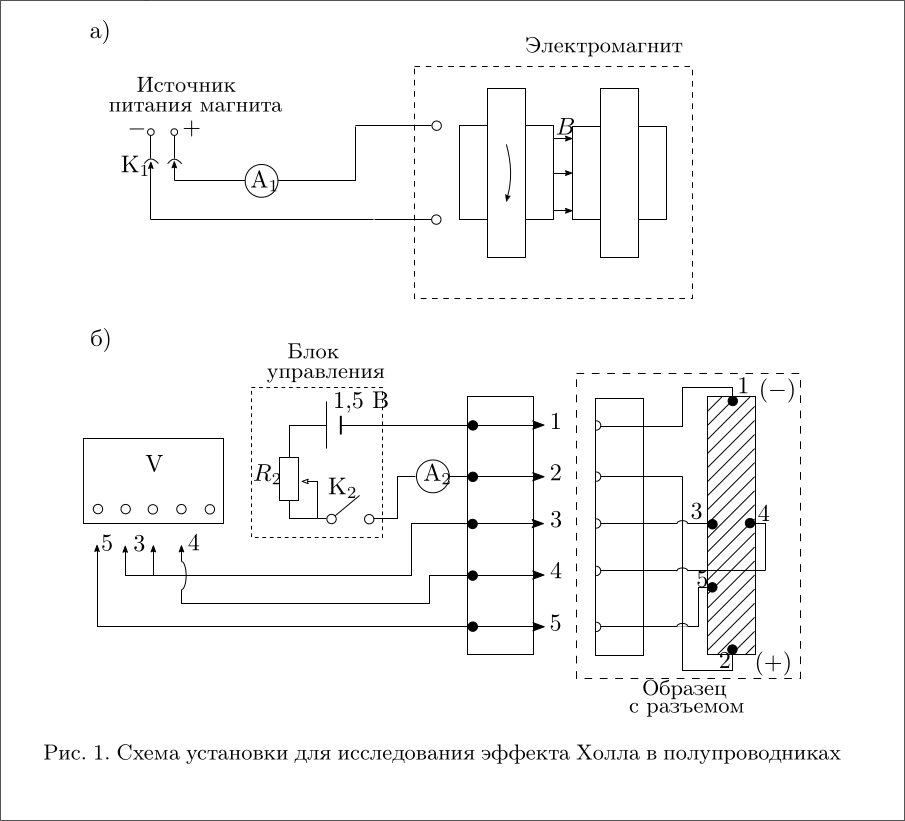
\includegraphics[width=1\textwidth]{img/Setup.png}
    \end{subfigure}
\end{figure}

Однако контакты 3 и 4 могут лежать не на одной эквипотенциали, поэтому напряжение
между ними является суммой омического падения напряжения и ЭДС Холла.

\begin{equation}
    U_{34} = \varepsilon_\text{Холла} + U_0
\end{equation}

\begin{equation}
    \varepsilon_\text{Холла} = U_{34} - U_0
\end{equation}

Затем вольтметр ставится на контакты 3 и 5. Таким образом,
зная $I$ и $U_{35}$ можно найти удельное сопротивление образца.

\centering
\begin{tabular}{|c|c|}
    \toprule
    $Isc \text{, } \text{mA}$ & $U_{35} \text{, } \text{mV}$ \\
    \midrule
    1 & 2.657 \\
    \bottomrule
\end{tabular}

\begin{equation}
    \sigma =\frac{I_{sc}L}{U_{35}la} =
    146.64 \cdot (\text{Ом} \cdot \text{м})^{-1}
    \text{,}
\end{equation}
где $L$ - длина образца, $l$ - ширина, $a$ - толщина.

\subsection*{Результаты}

Для начала проградуируем наш магнит, измерив зависимость $B(I)$.

\centering
\begin{tabular}{|r|r|r|r|r|r|r|}
    \toprule
     & $U$, $V$ & $I_m$, A & $B1$, mTl & $B2$, mTl & $B3$, mTl & $\overline{B}$, mTl \\
    \midrule
    $0$ & $21.10$  & $0.24$ & $234.20$  & $233.90$  & $233.70$  & $233.93$  \\
    $1$ & $39.30$  & $0.47$ & $447.10$  & $446.90$  & $448.70$  & $447.57$  \\
    $2$ & $60.00$  & $0.71$ & $683.50$  & $684.00$  & $686.40$  & $684.63$  \\
    $3$ & $81.00$  & $0.96$ & $868.00$  & $869.10$  & $868.80$  & $868.63$  \\
    $4$ & $101.40$ & $1.20$ & $983.30$  & $985.10$  & $986.20$  & $984.87$  \\
    $5$ & $115.10$ & $1.36$ & $1042.50$ & $1045.90$ & $1044.60$ & $1044.33$ \\
    \bottomrule
\end{tabular}

\begin{figure}[H]
    \centering
    \begin{subfigure}{0.8\textwidth}
        \centering
        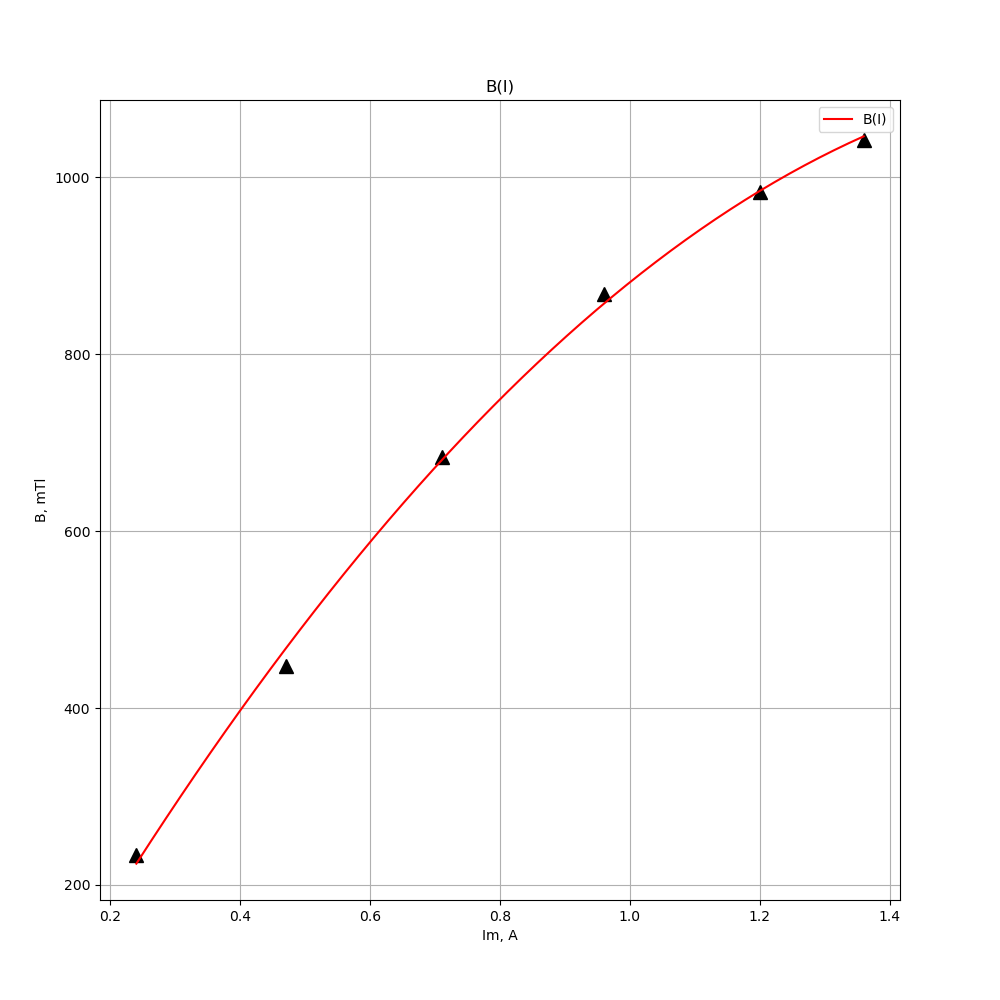
\includegraphics[width=0.8\textwidth]{img/B(I).png}
    \end{subfigure}
\end{figure}

По МНК приближаем эту кривую к квадратичной:

\begin{equation}
    B(I_m) = -362.82I_m^2 + 1314.38I_m - 70.43
\end{equation}

\raggedright
Далее снимем зависимости $\varepsilon_\text{Холла}(I_m)$ для
разных токов через наш образец, $I_{sc}$ - ток в образце,
$U_0$ - напряжение на контактак 3, 4 вне поля:

\begin{figure}[ht]
    \centering

    % First table
    \begin{subfigure}[b]{0.45\textwidth}
        \centering
        \begin{tabular}{|r|r|r|r|r|}
        \toprule
        U0, mV & Im, A & U34, mV & $\varepsilon_\text{Холла}, mV$ \\
        \midrule
        -0.02 & 0.24 & 0.00 & 0.02 \\
        -0.02 & 0.47 & 0.01 & 0.03 \\
        -0.02 & 0.71 & 0.03 & 0.05 \\
        -0.02 & 0.96 & 0.03 & 0.05 \\
        -0.02 & 1.20 & 0.04 & 0.06 \\
        -0.02 & 1.36 & 0.04 & 0.06 \\
        \bottomrule
        \end{tabular}
        \caption{$Isc = 0.14, mA$}
    \end{subfigure}
    \hfill
    % Second table
    \begin{subfigure}[b]{0.45\textwidth}
        \centering
        \begin{tabular}{|r|r|r|r|r|}
        \toprule
        U0, mV & Im, A & U34, mV & $\varepsilon_\text{Холла}, mV$ \\
        \midrule
        -0.03 & 0.24 & 0.00 & 0.03 \\
        -0.03 & 0.47 & 0.03 & 0.06 \\
        -0.03 & 0.71 & 0.06 & 0.09 \\
        -0.03 & 0.96 & 0.07 & 0.10 \\
        -0.03 & 1.20 & 0.09 & 0.12 \\
        -0.03 & 1.36 & 0.09 & 0.12 \\
        \bottomrule
        \end{tabular}
        \caption{$Isc = 0.31, mA$}
    \end{subfigure}

    % Third table
    \begin{subfigure}[b]{0.45\textwidth}
        \centering
        \begin{tabular}{|r|r|r|r|r|}
        \toprule
        U0, mV & Im, A & U34, mV & $\varepsilon_\text{Холла}, mV$ \\
        \midrule
        -0.05 & 0.24 & 0.00 & 0.05 \\
        -0.05 & 0.47 & 0.05 & 0.10 \\
        -0.05 & 0.71 & 0.09 & 0.14 \\
        -0.05 & 0.96 & 0.12 & 0.17 \\
        -0.05 & 1.20 & 0.14 & 0.19 \\
        -0.05 & 1.35 & 0.14 & 0.19 \\
        \bottomrule
        \end{tabular}
        \caption{$Isc = 0.48, mA$}
    \end{subfigure}
    \hfill
    % Fourth table
    \begin{subfigure}[b]{0.45\textwidth}
        \centering
        \begin{tabular}{|r|r|r|r|r|}
        \toprule
        U0, mV & Im, A & U34, mV & $\varepsilon_\text{Холла}, mV$ \\
        \midrule
        -0.07 & 0.24 & 0.01 & 0.08 \\
        -0.07 & 0.47 & 0.06 & 0.13 \\
        -0.07 & 0.71 & 0.12 & 0.19 \\
        -0.07 & 0.96 & 0.16 & 0.23 \\
        -0.07 & 1.20 & 0.18 & 0.25 \\
        -0.07 & 1.35 & 0.20 & 0.27 \\
        \bottomrule
        \end{tabular}
        \caption{$Isc = 0.65, mA$}
    \end{subfigure}

    % Fifth table
    \begin{subfigure}[b]{0.45\textwidth}
        \centering
        \begin{tabular}{|r|r|r|r|r|}
        \toprule
        U0, mV & Im, A & U34, mV & $\varepsilon_\text{Холла}, mV$ \\
        \midrule
        -0.09 & 0.24 & 0.01 & 0.10 \\
        -0.09 & 0.47 & 0.08 & 0.17 \\
        -0.09 & 0.71 & 0.15 & 0.24 \\
        -0.09 & 0.96 & 0.20 & 0.29 \\
        -0.09 & 1.20 & 0.23 & 0.32 \\
        -0.09 & 1.34 & 0.25 & 0.34 \\
        \bottomrule
        \end{tabular}
        \caption{$Isc = 0.82, mA$}
    \end{subfigure}
    \hfill
    % Sixth table
    \begin{subfigure}[b]{0.45\textwidth}
        \centering
        \begin{tabular}{|r|r|r|r|r|}
        \toprule
        U0, mV & Im, A & U34, mV & $\varepsilon_\text{Холла}, mV$ \\
        \midrule
        -0.11 & 0.24 & 0.01 & 0.12 \\
        -0.11 & 0.47 & 0.10 & 0.21 \\
        -0.11 & 0.71 & 0.19 & 0.30 \\
        -0.11 & 0.96 & 0.24 & 0.35 \\
        -0.11 & 1.20 & 0.28 & 0.39 \\
        -0.11 & 1.34 & 0.30 & 0.41 \\
        \bottomrule
        \end{tabular}
        \caption{$Isc = 0.99, mA$}
    \end{subfigure}

\end{figure}

\begin{figure}[H]
    \centering
    \begin{subfigure}{1.\textwidth}
        \centering
        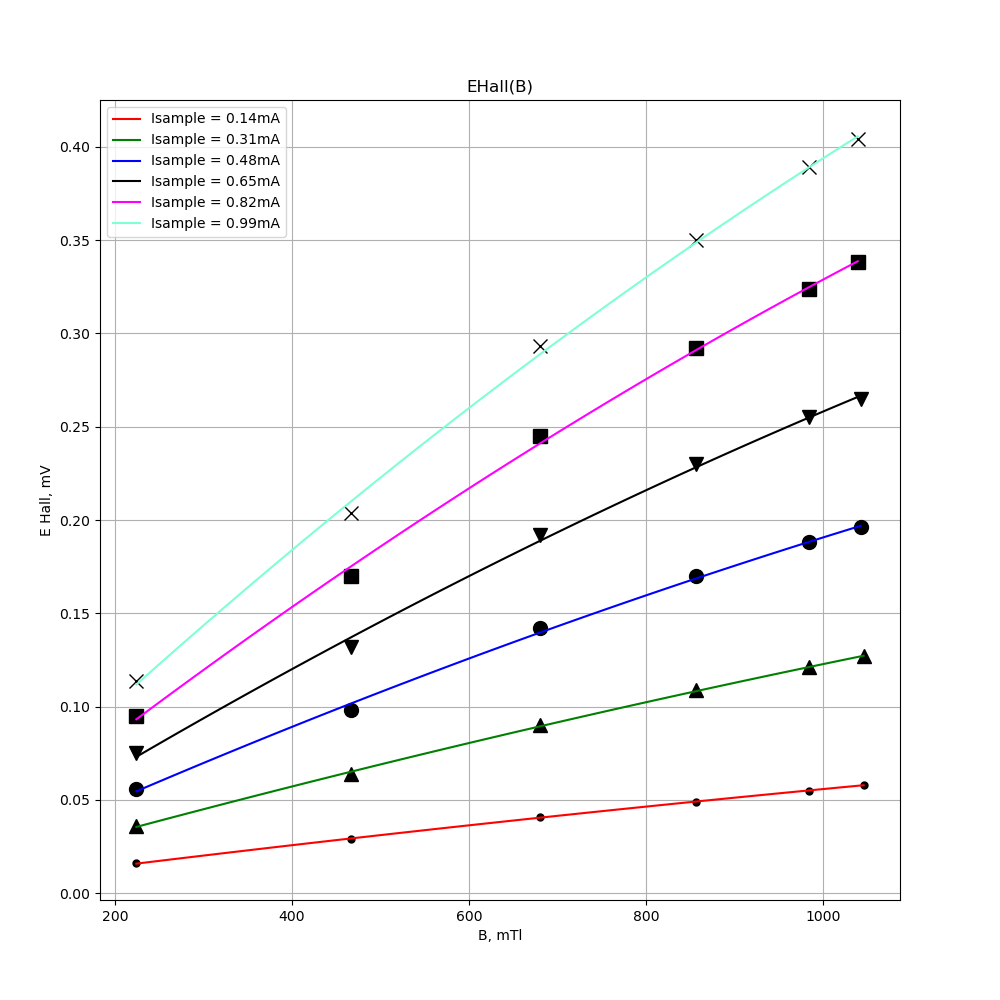
\includegraphics[width=1.\textwidth]{img/eHall(B).png}
    \end{subfigure}
\end{figure}

\begin{figure}[H]
    \centering
    \begin{tabular}{|r|r|r|r|r|r|}
        \toprule
        $I_{sc}, mA$ & $K, \frac{V}{Tl}$ & $\sigma_K, \frac{V}{Tl}$ & $\varepsilon_K, \frac{V}{Tl}$ \\
        \midrule
        0.14 & 5.10e-05 & 1.02e-06 & 0.02 \\
        0.31 & 1.11e-04 & 2.34e-06 & 0.02 \\
        0.48 & 1.73e-04 & 5.28e-06 & 0.03 \\
        0.65 & 2.35e-04 & 7.29e-06 & 0.03 \\
        0.82 & 3.00e-04 & 8.80e-06 & 0.02 \\
        0.99 & 3.59e-04 & 1.04e-05 & 0.02 \\
        \bottomrule
    \end{tabular}
\end{figure}

\begin{figure}[H]
    \centering
    \begin{subfigure}{1.\textwidth}
        \centering
        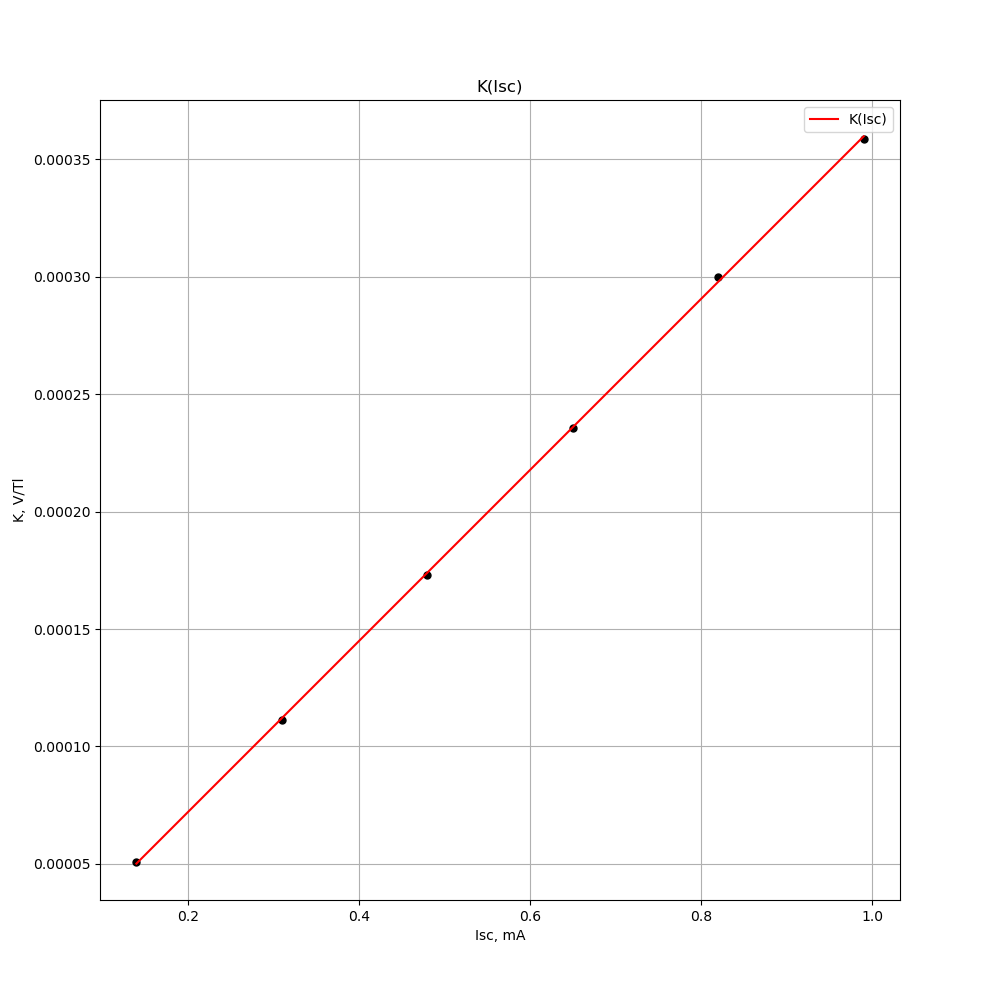
\includegraphics[width=1.\textwidth]{img/K(Isc).png}
    \end{subfigure}
\end{figure}

Наклон $k = \frac{dK}{dI_{sc}} = 3.64 \cdot 10^{-1}
\frac{\text{V}}{\text{TlA}} (\varepsilon_k = 0.5\%)$.

Согласно формуле 3.27:
\begin{equation}
    \varepsilon_\text{Холла} = R_h \cdot \frac{B}{a} \cdot I_{sc}
\end{equation}
Отсюда:
\begin{equation}
    R_h = ak = 8.01 \cdot 10^{-4} \frac{\text{м}^3}{\text{Кл}}
    (\varepsilon_{R_h} = \varepsilon_k = 0.5\%)
\end{equation}

\begin{equation}
    R_h = \frac{1}{nq} \implies n = \frac{1}{R_hq} = 7.80 \cdot 10^{21}
    \frac{1}{\text{м}^3}
    (\varepsilon_{n} = \varepsilon_{R_h} = 0.5\%)
\end{equation}

Так как $R_h$ положительные, а также по правилу левой руки можно сказать,
что в нашем образце дырочная проводимость.

\begin{equation}
    \sigma = qnb
\end{equation}
\begin{equation}
    b = \frac{\sigma}{qn} = \sigma R_h = 1.17 \cdot 10^{-1}
    \frac{\text{м}^2}{\text{В} \cdot \text{с}}
    = 1.17 \cdot 10^3 \frac{\text{см}^2}{\text{В} \cdot \text{с}}
    (\varepsilon_{b} = \varepsilon_{R_h} = 0.5\%)
\end{equation}

\centering
\begin{tabular}{|c|c|c|c|c|}
    \toprule
    $R_h \pm \Delta R_h$ & Знак носит. & $n \pm \Delta n$ & $\sigma \pm \Delta \sigma$ & $b \pm \Delta b$ \\
    $10^{-4} \text{м}^3/\text{Кл}$ & & $(\text{м}^3)^{-1}$ & $(\Omega \cdot \text{м})^{-1}$ & $\text{см}^2/(B \cdot c)$ \\
    \midrule
    $8.01 \pm 0.04$ & + & $7.80 \cdot 10^{21} \pm 3.9 \cdot 10^{19}$ & $146.64$ & $1.17 \cdot 10^3 \pm 5.85$ \\
    \bottomrule
\end{tabular}

\end{document}
